\documentclass{article}
\usepackage{tikz}
\usepackage{pgfplots}
\usepackage{xcolor}
\usepackage{svg}
\usepackage{amsmath}
\usepackage{array}
\usepackage[skins]{tcolorbox}
\usepackage[version=4]{mhchem}
\usepackage[a4paper, total={6in, 8in}]{geometry}
\usepackage{fouriernc}
\usepackage{xymtex}
\usepackage{textcomp}
\usepackage{eurosym}
\usepackage{caption}
\usepackage{longtable}


\title{Relazione - pendolo di Kater}
\author{Federico Cesari}
\date{gennaio 2024}




\begin{document}
	\maketitle
	\vspace{3cm}
	
	L'esperienza di laboratorio ha lo scopo di determinare il periodo di oscillazione di un pendolo fisico in presenza di errori casuali (ed eventualmente di errori sistematici) e verificare che le misure osservate sono accurate o meno rispetto alle misure della fotocellula.
	
	\vspace{0.5cm}
	\begin{table}[hb]
		\centering
		\renewcommand{\arraystretch}{1.5}
		\begin{tabular}{lr}
			 & \textit{sensibilità}\\
			 \hline
			Cronometro $\quad$                	& $0.01s$    \\
			Fotocellula  $\quad$                & $0.001s$    \\
		\end{tabular}
		\renewcommand{\arraystretch}{1}
		\captionof*{table}{\textbf{Strumenti}}
	\end{table}
	\vspace{0.5cm}
	
	\textit{descrivere brevemente la procedura di misura effettuata}
	
	
	
	
	
	
	
	
	
	\newpage
	\section{Punto 4}
	
	Dalle cento misure ho ricavato i valori nella prima tabella. Il più piccolo valore rilevato ($1.59s$) e il più grande ($2.31s$) decido di escluderli secondo il criterio di rigetto a $3\sigma$: so infatti che le mie misure hanno il $99.7 \%$ di probabilità di ricadere nell'intervallo $(\mu  - 3\sigma , \mu + 3\sigma)$, dove $\mu$ è la media della popolazione. Posso quindi affermare che valori osservati oltre $3 \sigma$ appartengono a un'altra popolazione e, di conseguenza, che è lecito rigettarli. \\ 
	
	\noindent
	Successivamente al rigetto, con i $98$ dati rimanenti ricavo i nuovi valori riportati nella seconda tabella.
	
	\vspace{0.8cm}
	\begin{minipage}[c]{0.45\textwidth}
		\centering
		\begin{tabular}{llrl}
			Media                       & $\bar{x}$             & $1.95$        & $s$       \\
			Varianza                    & $\sigma ^ 2$          & $0.0092$     & $s^2$  \\
			Dev. std                    & $\sigma$              & $0.096$      & $s$   \\
			Dev. std (della media)      & $\sigma_{\bar{x}}$    & $0.0096$     & $s$    \\
			Mediana                     & $\mu_e$               & $1.95$        &  $s$      \\
			Moda                        & $v_0$                 & $2.00$        & $s$
		\end{tabular}
		\captionof{table}{\textbf{100 misure}}
	\end{minipage}
	\begin{minipage}[c]{0.5\textwidth}
		\centering
		\begin{tabular}{llrl}
			Media                       & $\bar{x}$             & $1.95$        & $s$       \\
			Varianza                    & $\sigma ^ 2$          & $0.0068$     & $s^2$  \\
			Dev. std                    & $\sigma$              & $0.082$      & $s$   \\
			Dev. std (della media)      & $\sigma_{\bar{x}}$    & $0.0083$     & $s$    \\
			Mediana                     & $\mu_e$               & $1.95$        &  $s$      \\
			Moda                        & $v_0$                 & $2.00$        & $s$
		\end{tabular}
		\captionof{table}{\textbf{98 misure}}
	\end{minipage}
	\vspace{0.8cm}
	
	\noindent
	Confrontando i valori nelle due tabelle si notano una sensibile diminuzione della varianza ($-26 \%$) e una variazione della deviazione standard e della deviazione standard della media (entrambe circa $-13 \%$). Variazioni prevedibili vista l'esclusione di valori molto distanti dalla media della popolazione. 
	
	\vspace{0.8cm}
	\begin{table}[hb]
		\centering
		\begin{tabular}{llrl}
			Media                       & $\bar{x}$             & $1.95$        & $s$       \\
			Varianza                    & $\sigma ^ 2$          & $0.0067$     & $s^2$  \\
			Dev. std                    & $\sigma$              & $0.082$      & $s$   \\
			Dev. std (della media)      & $\sigma_{\bar{x}}$    & $0.0083$     & $s$    
		\end{tabular}
		\captionof{table}{\textbf{Dati accorpati}}
	\end{table}
	\vspace{0.5cm}
	
	\noindent
	I dati accorpati producono valori pressoché identici a quelli rilevati post rigetto a $3\sigma$. \\
	
	
	\noindent
	La sensibilità dello strumento è $0.01s$, ciò significa che lo strumento non può distinguere o rilevare variazioni inferiori a tale valore. La deviazione standard da me calcolata mi dice invece che le mie misure hanno una dispersione naturale attorno al valor medio uguale a $0.008s$, quindi minore della sensibilità dello strumento. Scelgo $0.01s$ come errore sulla stima, essendo questo il più piccolo valore misurabile. \\
	
	
	\noindent
	Dopo aver escluso i dati appartenenti a un'altra popolazione e raggruppato i dati, la mia migliore stima del  periodo di oscillazione del pendolo è:
	\[
	1.95s \quad \pm \quad 0.01 s
	\]
	
	
	
	
	
	\newpage
	\section{Test del $\chi ^2$}
	E' ragionevole pensare che le nostre misure siano governate da una distribuzione limite di tipo gaussiano centrata nel valore corrispendente alla mia migliore stima $\bar{x}$. Ci aspettiamo infatti che le misure siano soggette a errori sistematici
	
	\vspace{0.6cm}
	\begin{center}
	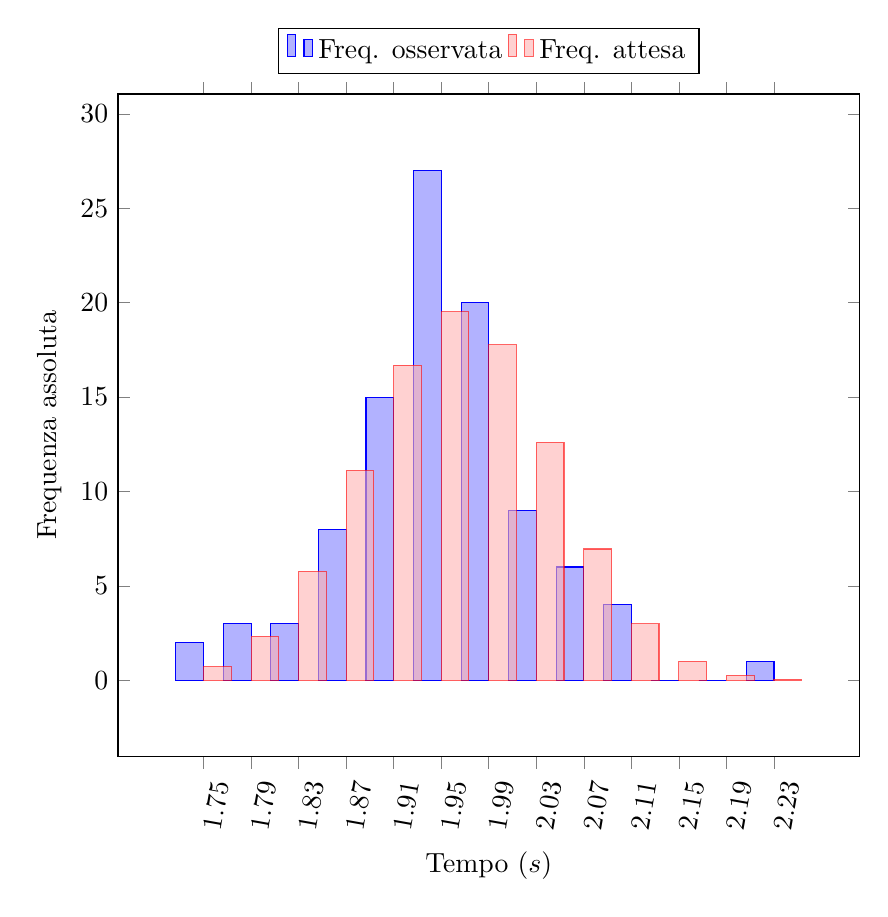
\begin{tikzpicture}
		\pgfplotsset{compat = 1.3}
		\begin{axis}[
			width=11cm, 
			height=10cm,
			ylabel=Frequenza assoluta,
			xlabel=Tempo $(s)$,
			enlargelimits=0.15,
			legend style={at={(0.5,1.1)},	anchor=north,legend columns=-1},
			ybar=0pt,% configures `bar shift'
			bar width=10pt,
			xtick={1.745,
				1.785,
				1.825,
				1.865,
				1.905,
				1.945,
				1.985,
				2.025,
				2.065,
				2.105,
				2.145,
				2.185,
				2.225},
			xticklabel style={rotate=80, anchor=north east}
			]
			\addplot+[opacity=1] 
			coordinates {
			(1.745,2)
			(1.785,3)
			(1.825,3)
			(1.865,8)
			(1.905,15)
			(1.945,27)
			(1.985,20)
			(2.025,9)
			(2.065,6)
			(2.105,4)
			(2.145,0)
			(2.185,0)
			(2.225,1)};
			\addplot+[opacity=0.6]
			coordinates {
			(1.745,0.733)
			(1.785,2.330)
			(1.825,5.767)
			(1.865,11.116)
			(1.905,16.688)
			(1.945,19.510)
			(1.985,17.764)
			(2.025,12.597)
			(2.065,6.957)
			(2.105,2.992)
			(2.145,1.002)
			(2.185,0.261)
			(2.225,0.053)
			};
			\legend{Freq. osservata,Freq. attesa}
		\end{axis}
	\end{tikzpicture}
	\end{center}
	
	\newpage
	\section{Punto 6}
	
	\newpage
	\section{Punto 7}
	\newpage
	\section{Punto 8}
	
	\newpage
	\section{Punto 9}
	
	
	
\end{document}
